

\section{Sensor Indutivo}
\label{indutivo}


\begin{table}[ht!]

	\begin{tabular}{r l|l p{12cm} }
		
		\textcolor{gray}{Especificação} &&& 	{Sensor Indutivo - NBB20-L2-E2-V1 }\\
		\textcolor{gray}{Data} &&& 				{08/04/2014 e 28/11/2014}\\
        \textcolor{gray}{Beneficiado} &&&		{Pepperl Fuchs Ltda} \\
        \textcolor{gray}{CNPJ} &&& 				{64.126.675/0001-64} \\
        \textcolor{gray}{Número Nota} &&& 		{40885 e 49075} \\
		\textcolor{gray}{Quantidade} &&& 		{6} \\
		\textcolor{gray}{Valor} &&& 			{R\$379,03 + R\$455,27} \\
		\textcolor{gray}{Data Sheet} &&& 		{Anexo II - \ref{datasheet_indutivo} } \\

		\textcolor{gray}{Função no projeto} &&& {O sensor indutivo será utilizado para detectar o contato entre a garra pescadora e o Stoplog, verificando assim se o mesmo está corretamente enganchado. } \\
		\textcolor{gray}{Razão da Escolha} &&& {Os fornecedores pesquisados para sensores indutivos que atendem aos requisitos de projeto são: Contrinex, Pepperl-Fuchs e Turck. Diversos modelos foram avaliados, juntamente com os técnicos das respectivas empresas. A lista dos modelos de cada fabricante que seriam ideais à aplicação no projeto se encontra na tabela abaixo. Por os modelos serem equivalente em aplicabilidade, foi selecionado o sensor que apresenta o menor custo ao projeto o NBB20-L2-E2-V1. Os sensores indutivos serão instalados nas garras pescadoras e serão conectados a eletrônica embarcada, sendo a distância entre os itens de até 5 mestro, depenendo do modelo de garra pescador. Logo, a necessidade da compra do cabo. 
		\begin{itemize}
		  \item \textbf {NBB20-L2-E2-V1 da Pepperl Fuchs  por R\$131,37}
		  \item NI35-CP40-VP4X2 da TURCK por R\$ 428,97 
		  \item NI50-Q42 da TURCK por R\$ 414,75
		\end{itemize}}
		

	\end{tabular}
\end{table}

\newpage

\subsection{Foto do Material}
\begin{figure}[H]
 \centering
 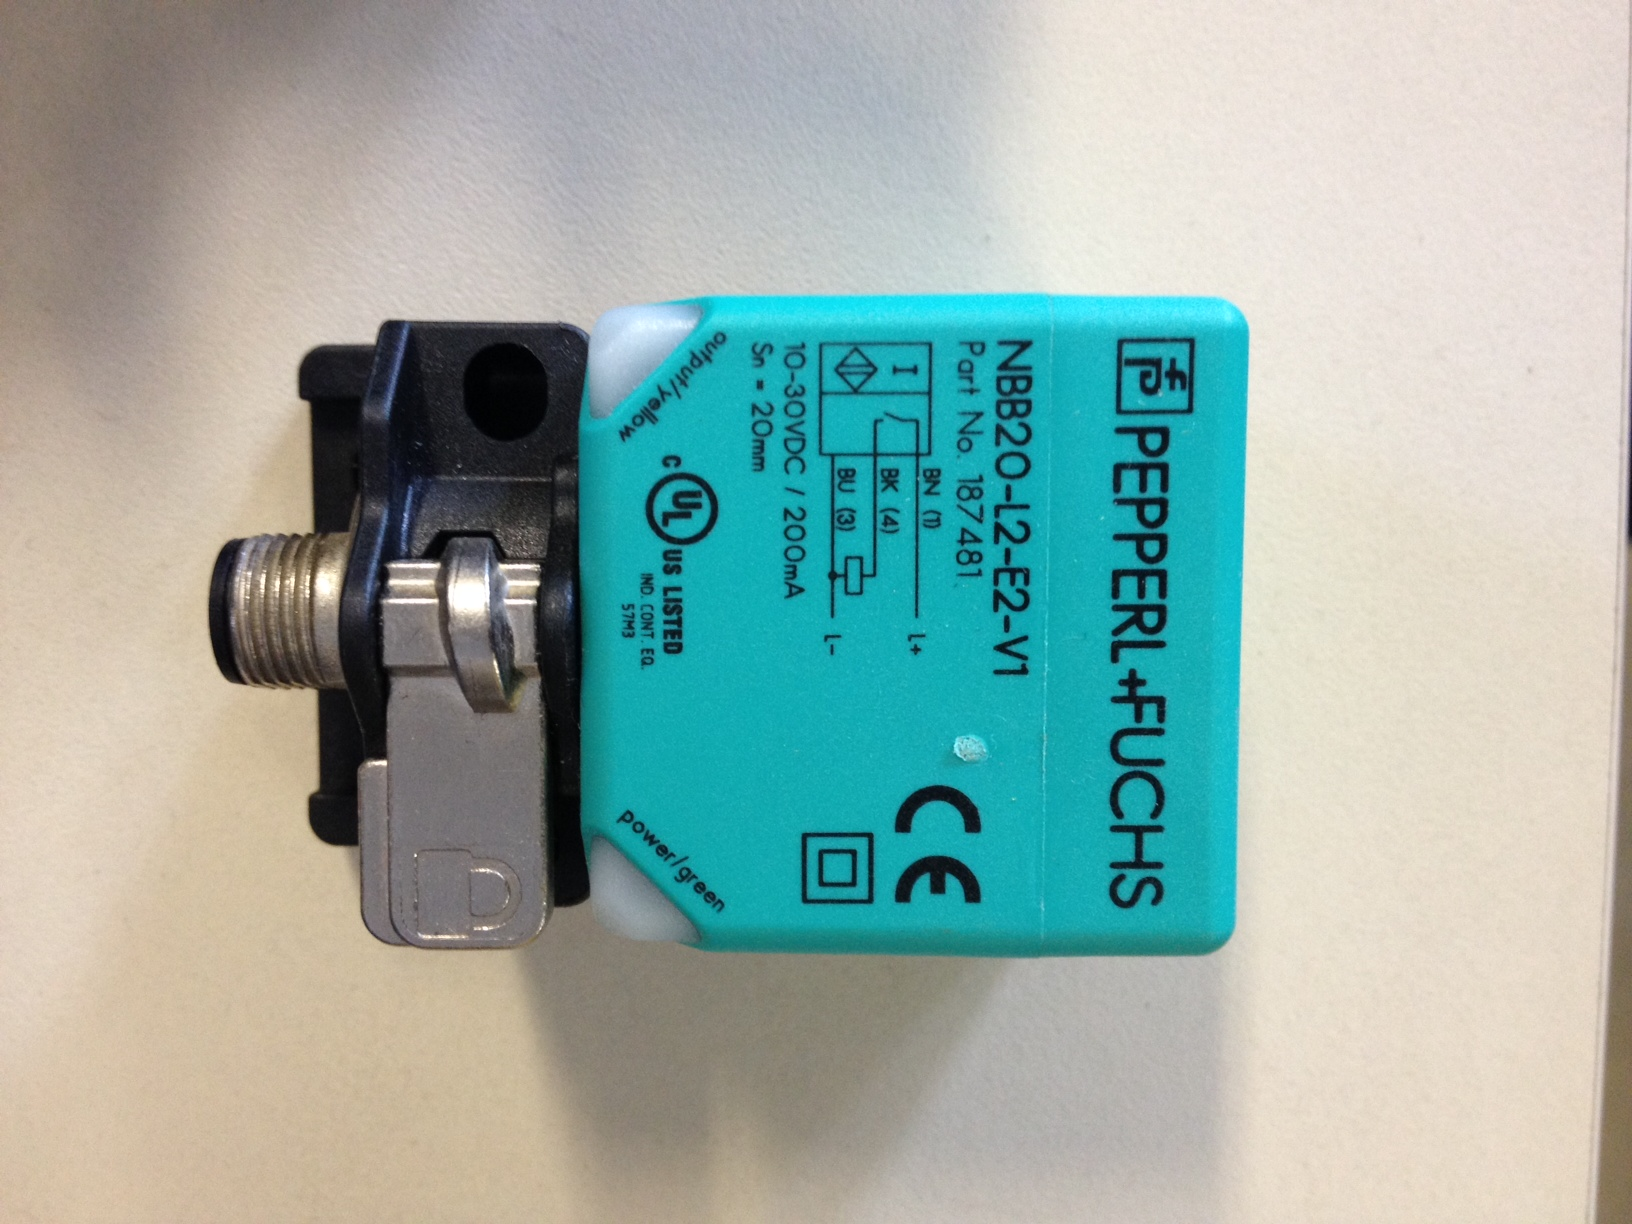
\includegraphics[width=1\columnwidth]{Indutivo/foto}
 \caption{Sensor Indutivo - NBB20-L2-E2-V1 }
\end{figure}
\newpage

\subsection{Cotação Sensor Indutivo 1 }
\begin{figure}[H]
 \centering
 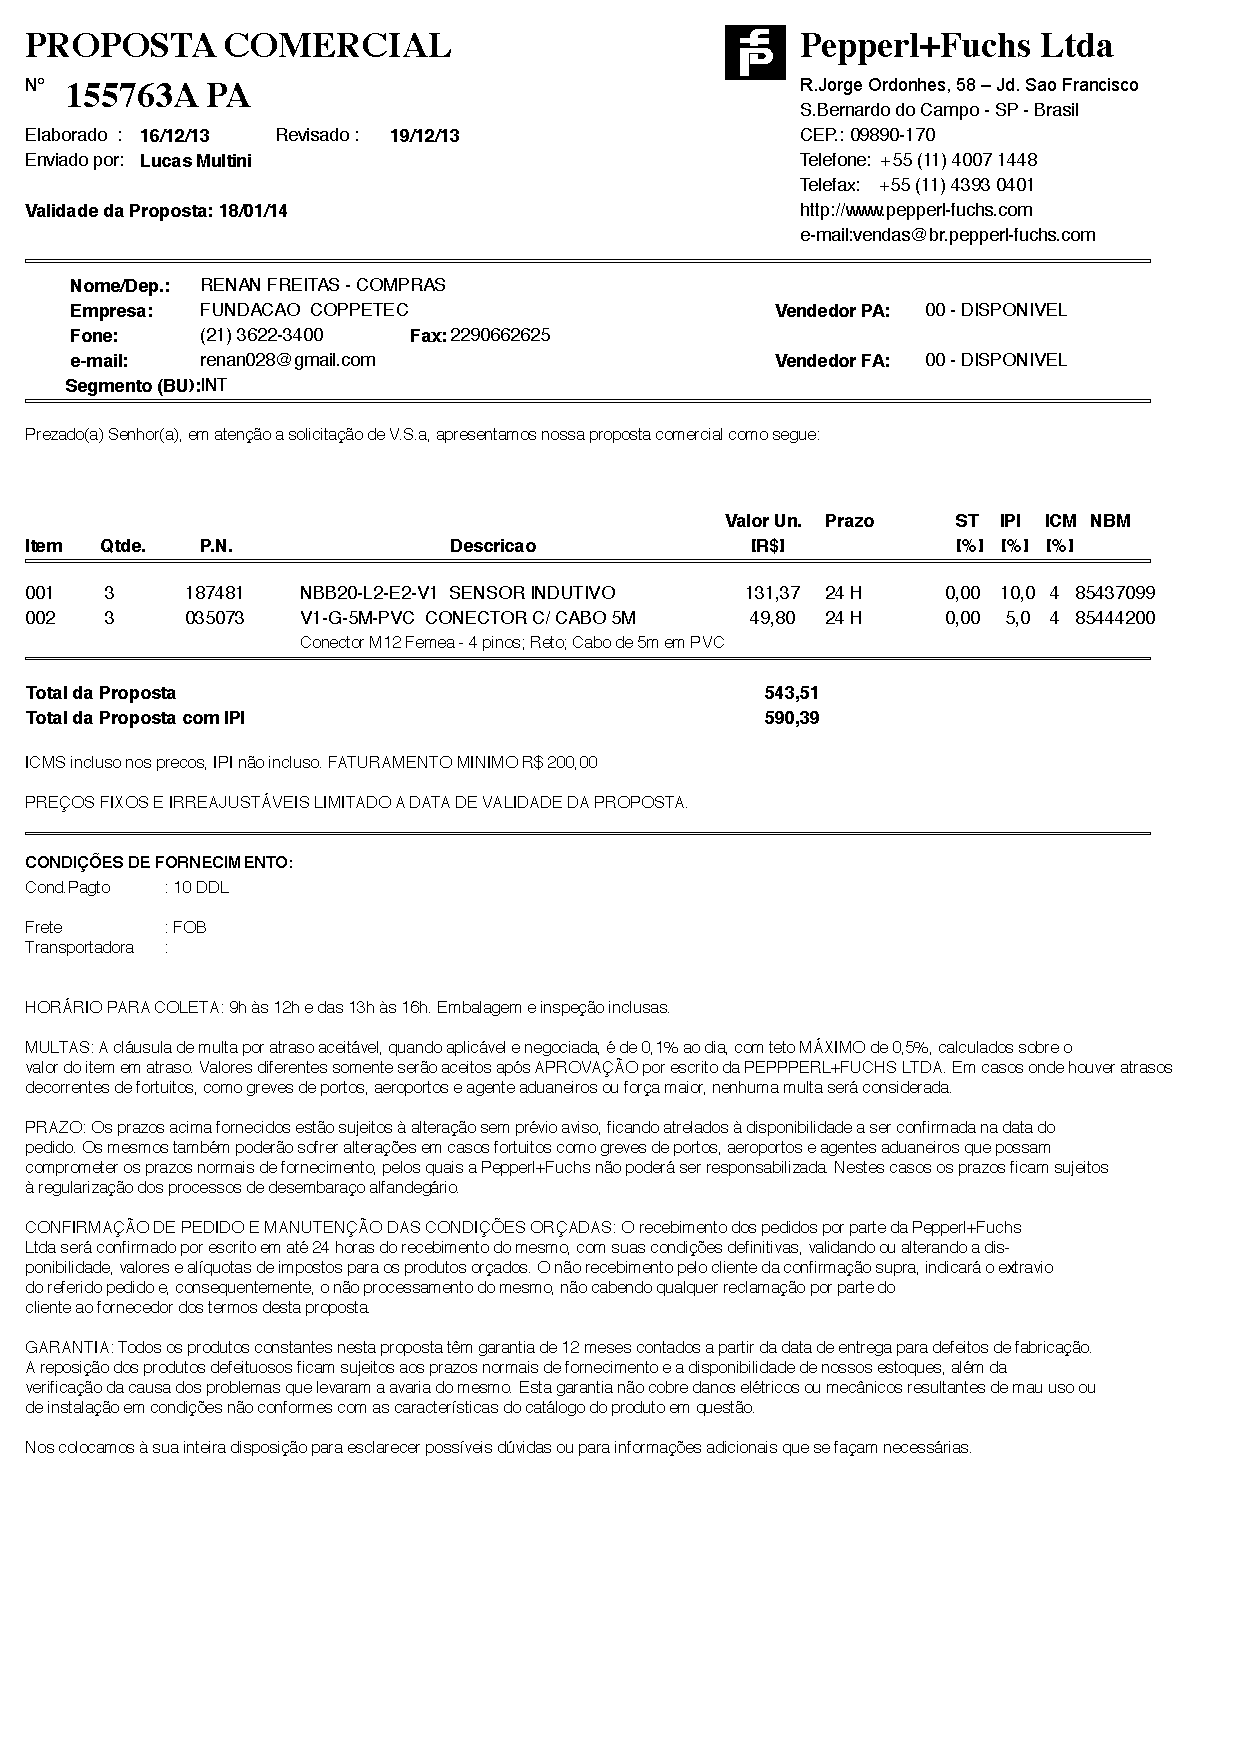
\includegraphics[width=1\columnwidth]{Indutivo/price_quote_0.pdf}
 \caption{Cotação Sensor Indutivo - NBB20-L2-E2-V1 }
\end{figure}

\subsection{Cotação Sensor Indutivo 2 }
\begin{figure}[H]
 \centering
 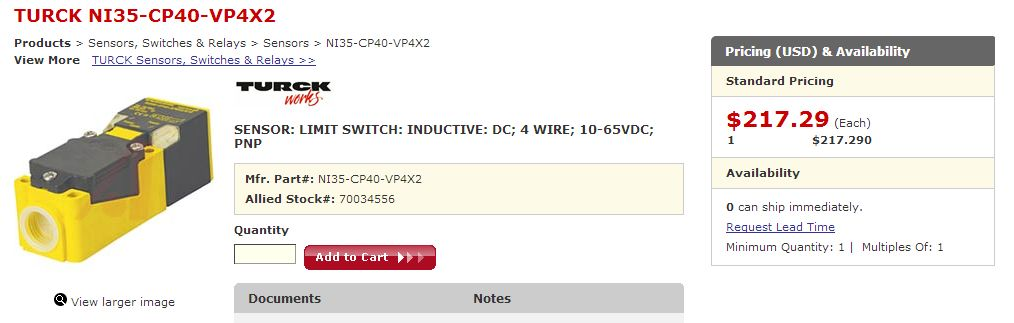
\includegraphics[width=1\columnwidth]{Indutivo/price_quote_1}
 \caption{Cotação NI35-CP40-VP4X2 da TURCK}
\end{figure}

\subsection{Cotação Sensor Indutivo 3 }
\begin{figure}[H]
 \centering
 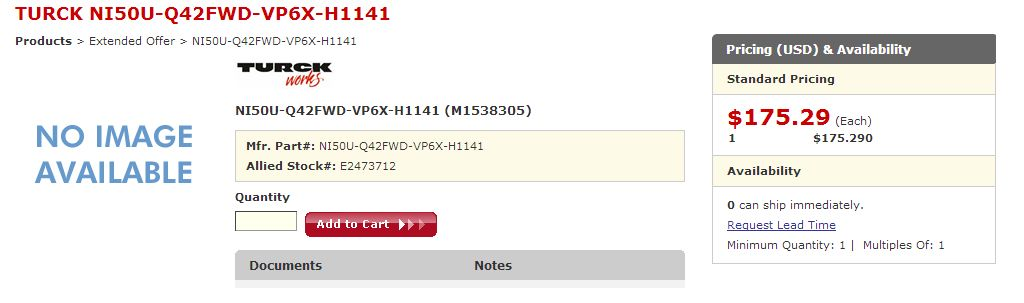
\includegraphics[width=1\columnwidth]{Indutivo/price_quote_2}
 \caption{Cotação NI50-Q42 da TURCK }
\end{figure}

\subsection{Nota Fiscal 1}
\begin{figure}[H]
 \centering
 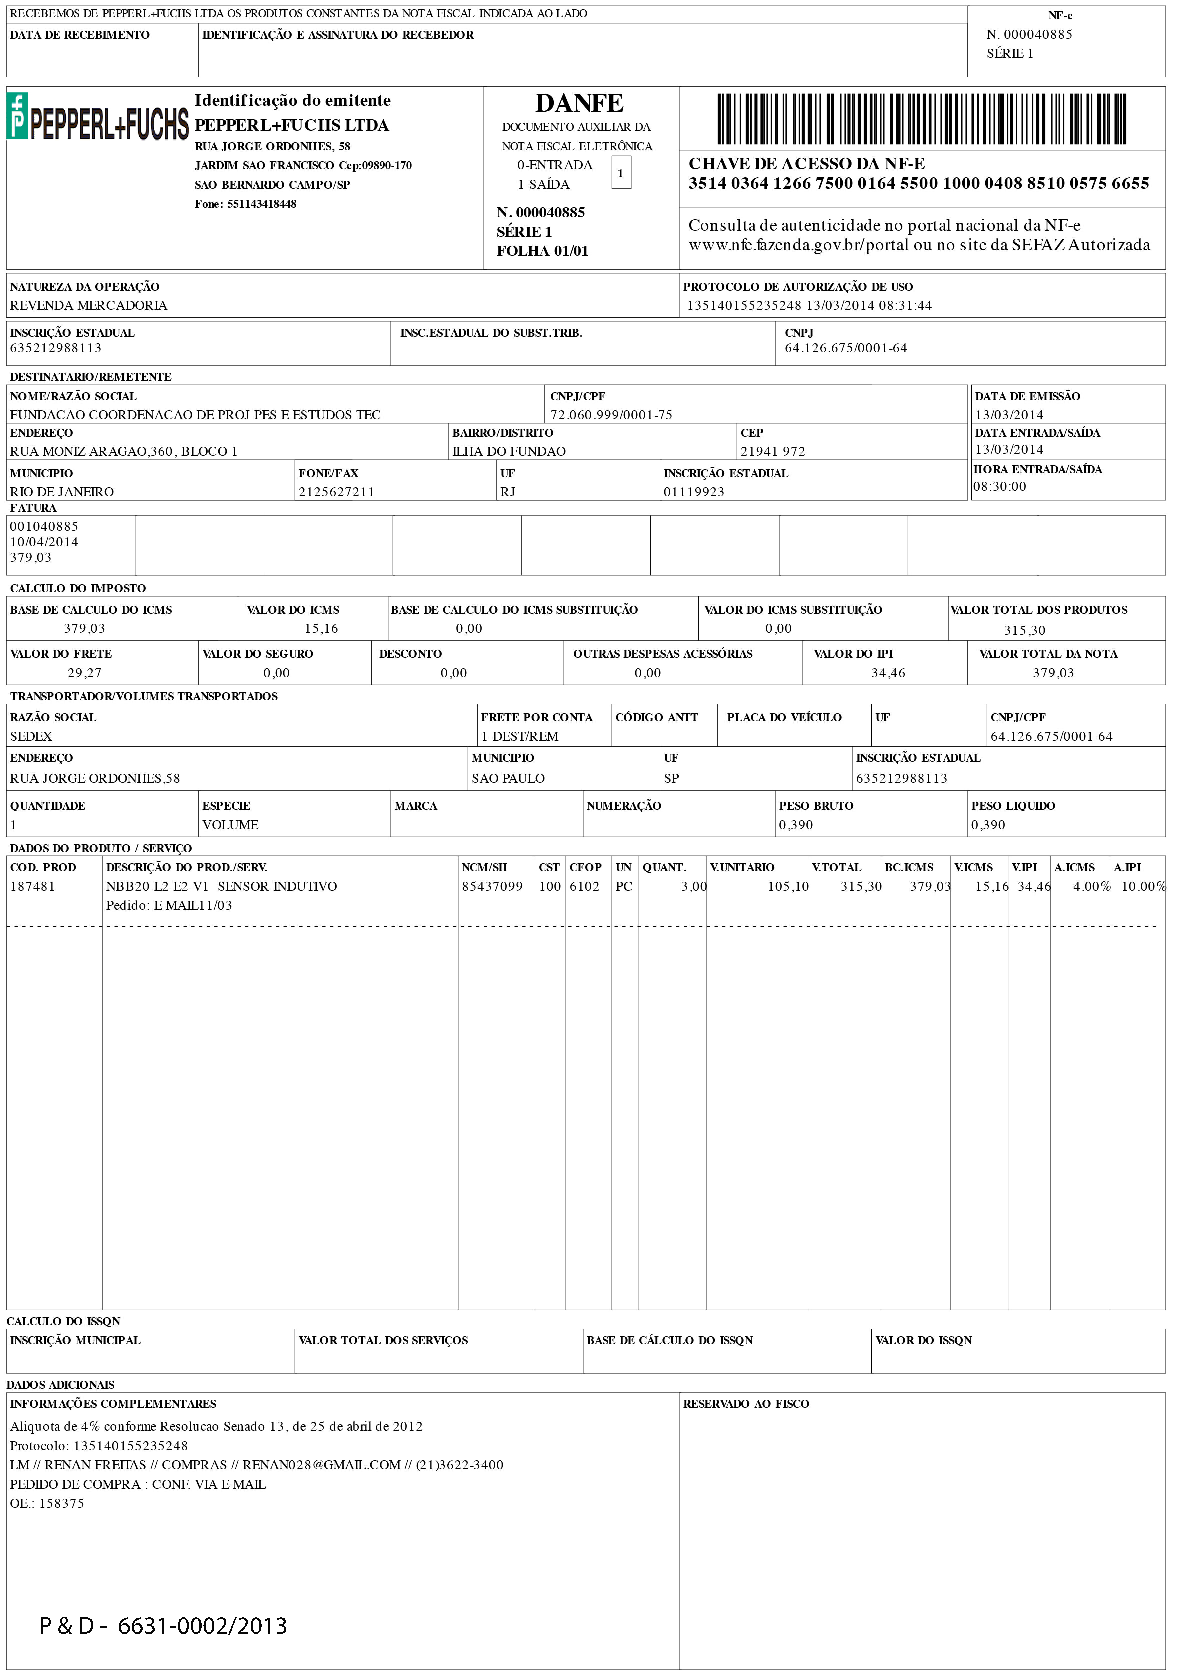
\includegraphics[width=1\columnwidth]{Indutivo/nota_indutivo.pdf}
 \caption{Nota Sensor Indutivo - NBB20-L2-E2-V1}
 \end{figure}
 
 \subsection{Nota Fiscal 2}
\begin{figure}[H]
 \centering
 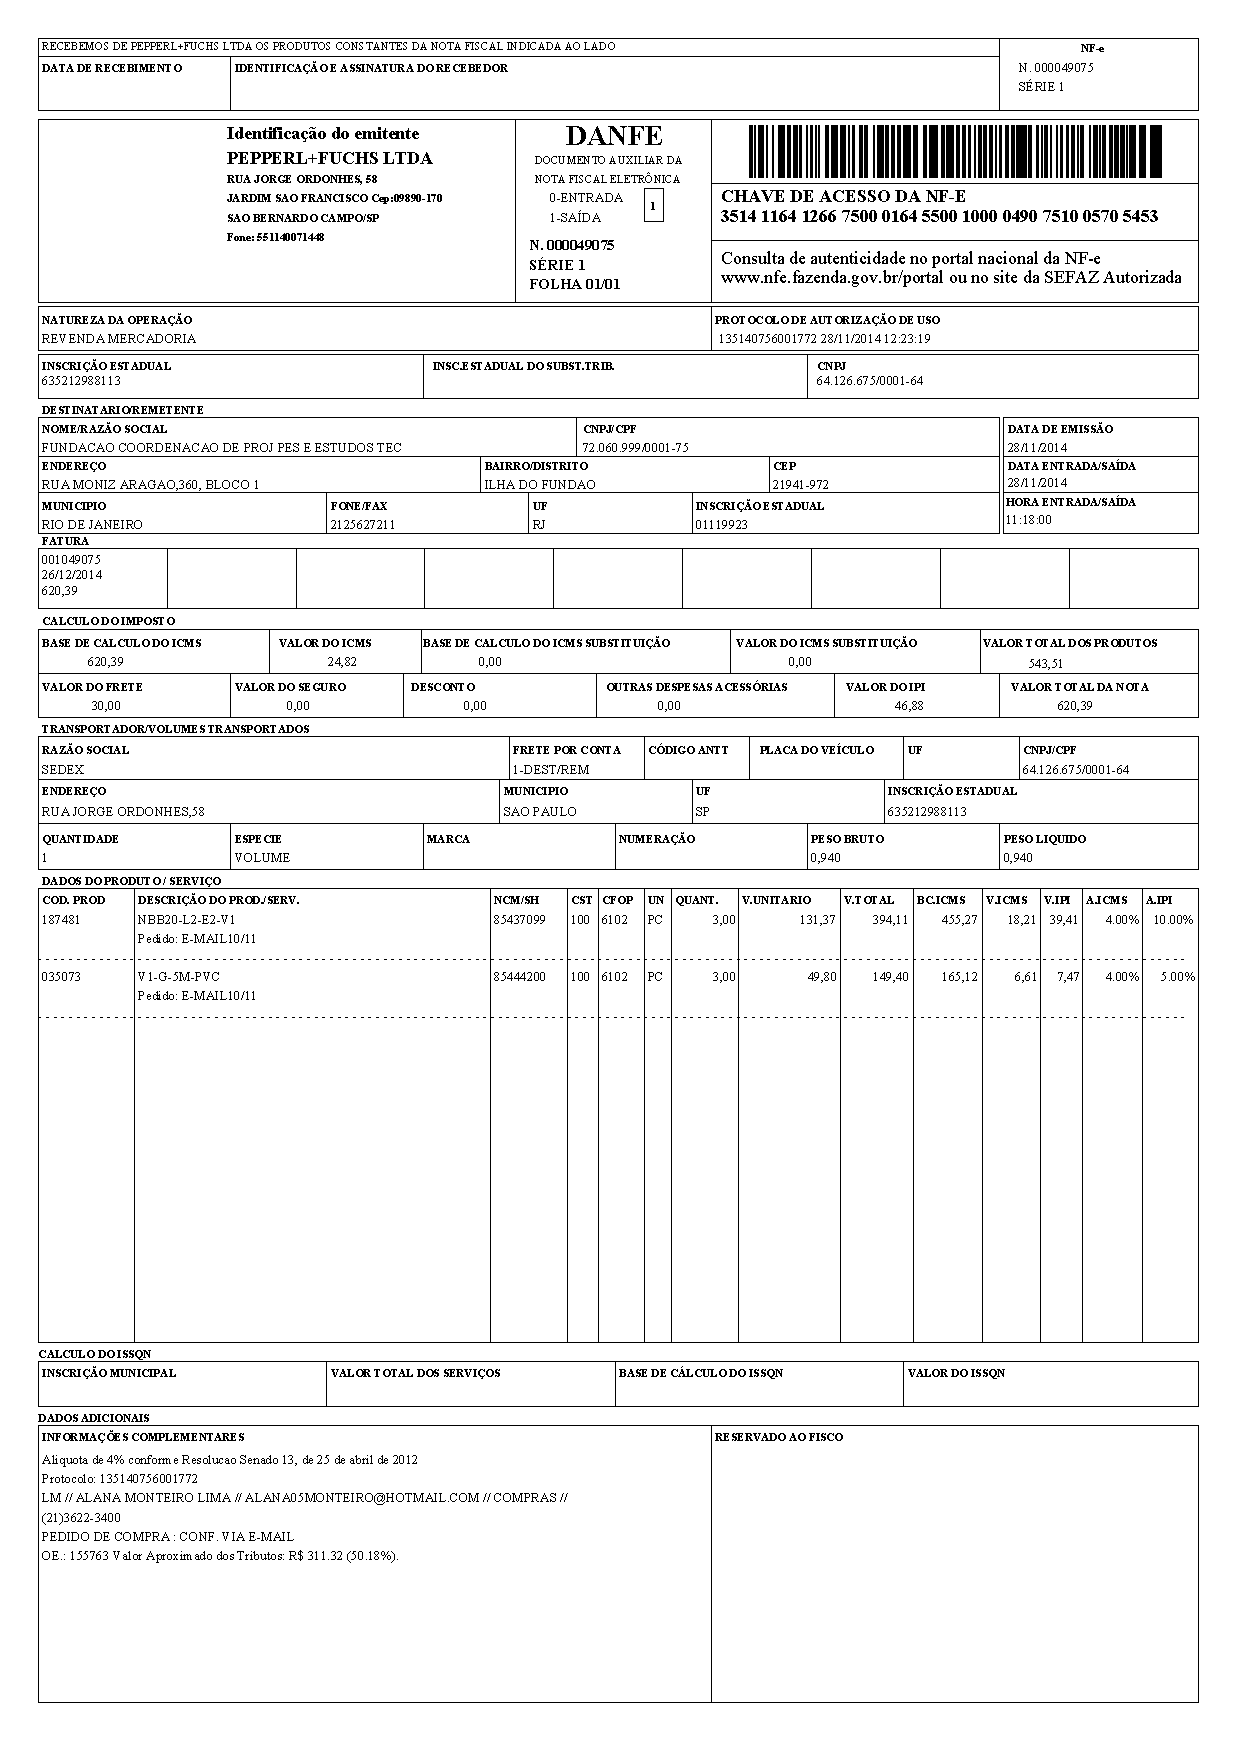
\includegraphics[width=0.9\columnwidth]{Indutivo/nota_indutivo2.pdf}
 \caption{Nota Sensor Indutivo 2 - NBB20-L2-E2-V1}
 \end{figure}